% Options for packages loaded elsewhere
\PassOptionsToPackage{unicode}{hyperref}
\PassOptionsToPackage{hyphens}{url}
%
\documentclass[
  ignorenonframetext,
  aspectratio=169,
]{beamer}
\usepackage{pgfpages}
\setbeamertemplate{caption}[numbered]
\setbeamertemplate{caption label separator}{: }
\setbeamertemplate{navigation symbols}{}
\setbeamertemplate{footline}[page number]
\setbeamercolor{caption name}{fg=normal text.fg}
\beamertemplatenavigationsymbolsempty
% Prevent slide breaks in the middle of a paragraph
\widowpenalties 1 10000
\raggedbottom
\setbeamertemplate{part page}{
  \centering
  \begin{beamercolorbox}[sep=16pt,center]{part title}
    \usebeamerfont{part title}\insertpart\par
  \end{beamercolorbox}
}
\setbeamertemplate{section page}{
  \centering
  \begin{beamercolorbox}[sep=12pt,center]{part title}
    \usebeamerfont{section title}\insertsection\par
  \end{beamercolorbox}
}
\setbeamertemplate{subsection page}{
  \centering
  \begin{beamercolorbox}[sep=8pt,center]{part title}
    \usebeamerfont{subsection title}\insertsubsection\par
  \end{beamercolorbox}
}
\AtBeginPart{
  \frame{\partpage}
}
\AtBeginSection{
  \ifbibliography
  \else
    \frame{\sectionpage}
  \fi
}
\AtBeginSubsection{
  \frame{\subsectionpage}
}
\usepackage{amsmath,amssymb}
\usepackage{lmodern}
\usepackage{iftex}
\ifPDFTeX
  \usepackage[T1]{fontenc}
  \usepackage[utf8]{inputenc}
  \usepackage{textcomp} % provide euro and other symbols
\else % if luatex or xetex
  \ifXeTeX
    \usepackage{xltxtra} 
    \usepackage{xeCJK}
    \setCJKmainfont{ipaexm.ttf}
    \setCJKsansfont{ipaexg.ttf}
    \setCJKmonofont{ipaexg.ttf}
  \fi
  \usepackage{unicode-math}
  \defaultfontfeatures{Scale=MatchLowercase}
  \defaultfontfeatures[\rmfamily]{Ligatures=TeX,Scale=1}
\fi
% Use upquote if available, for straight quotes in verbatim environments
\IfFileExists{upquote.sty}{\usepackage{upquote}}{}
\IfFileExists{microtype.sty}{% use microtype if available
  \usepackage[]{microtype}
  \UseMicrotypeSet[protrusion]{basicmath} % disable protrusion for tt fonts
}{}
\makeatletter
\@ifundefined{KOMAClassName}{% if non-KOMA class
  \IfFileExists{parskip.sty}{%
    \usepackage{parskip}
  }{% else
    \setlength{\parindent}{0pt}
    \setlength{\parskip}{6pt plus 2pt minus 1pt}}
}{% if KOMA class
  \KOMAoptions{parskip=half}}
\makeatother
\usepackage{xcolor}
\IfFileExists{xurl.sty}{\usepackage{xurl}}{} % add URL line breaks if available
\IfFileExists{bookmark.sty}{\usepackage{bookmark}}{\usepackage{hyperref}}
\hypersetup{
  pdftitle={Charitable Giving, Tax Reform, and Self-selection of Tax Report: Evidence from South Korea},
  hidelinks,
  pdfcreator={LaTeX via pandoc}}
\urlstyle{same} % disable monospaced font for URLs

\usepackage{setspace}
\usepackage{float}

\newif\ifbibliography
\usepackage{longtable,booktabs,array}
\usepackage{threeparttable, threeparttablex, multirow}
\usepackage{calc} % for calculating minipage widths
\usepackage{caption}
% Make caption package work with longtable
\makeatletter
\def\fnum@table{\tablename~\thetable}
\makeatother
\usepackage{graphicx}
\makeatletter
\def\maxwidth{\ifdim\Gin@nat@width>\linewidth\linewidth\else\Gin@nat@width\fi}
\def\maxheight{\ifdim\Gin@nat@height>\textheight\textheight\else\Gin@nat@height\fi}
\makeatother
% Scale images if necessary, so that they will not overflow the page
% margins by default, and it is still possible to overwrite the defaults
% using explicit options in \includegraphics[width, height, ...]{}
\setkeys{Gin}{width=\maxwidth,height=\maxheight,keepaspectratio}
% Set default figure placement to htbp
\makeatletter
\def\fps@figure{htbp}
\makeatother
\setlength{\emergencystretch}{3em} % prevent overfull lines
\providecommand{\tightlist}{%
  \setlength{\itemsep}{0pt}\setlength{\parskip}{0pt}}
\setcounter{secnumdepth}{-\maxdimen} % remove section numbering
\newlength{\cslhangindent}
\setlength{\cslhangindent}{1.5em}
\newlength{\csllabelwidth}
\setlength{\csllabelwidth}{3em}
\newlength{\cslentryspacingunit} % times entry-spacing
\setlength{\cslentryspacingunit}{\parskip}
\newenvironment{CSLReferences}[2] % #1 hanging-ident, #2 entry spacing
 {% don't indent paragraphs
  \setlength{\parindent}{0pt}
  % turn on hanging indent if param 1 is 1
  \ifodd #1
  \let\oldpar\par
  \def\par{\hangindent=\cslhangindent\oldpar}
  \fi
  % set entry spacing
  \setlength{\parskip}{#2\cslentryspacingunit}
 }%
 {}
\usepackage{calc}
\newcommand{\CSLBlock}[1]{#1\hfill\break}
\newcommand{\CSLLeftMargin}[1]{\parbox[t]{\csllabelwidth}{#1}}
\newcommand{\CSLRightInline}[1]{\parbox[t]{\linewidth - \csllabelwidth}{#1}\break}
\newcommand{\CSLIndent}[1]{\hspace{\cslhangindent}#1}
\ifLuaTeX
  \usepackage{selnolig}  % disable illegal ligatures
\fi

\title{Charitable Giving, Tax Reform, and Self-selection of Tax Report: Evidence from South Korea}


            \author[shortname]{ Hiroki Kato  Tsuyoshi Goto  Yong-Rok Kim }
            \institute[shortinst]{ \inst{} Osaka University \and  \inst{} Chiba University \and  \inst{} Kobe University \and }
  
\date{2021/07/25}


\begin{document}
\frame{\titlepage}

\hypertarget{introduction}{%
\section{Introduction}\label{introduction}}

\begin{frame}{Charitable Giving and Taxiation}
\protect\hypertarget{charitable-giving-and-taxiation}{}
In many countries, governments set a tax relief for charitable giving.

To evaluate the effect of tax relief, many papers investigate the elasticity of charitable donations with respect to their tax price (Almunia et al., 2020; Auten et al., 2002; Bakija and Heim, 2011; Fack and Landais, 2010; Randolph, 1995).

Focusing on the tax deduction or tax credit on the charity, they show that the price elasticity of giving is about -1 or more in terms of absolute value.
\end{frame}

\begin{frame}{Charitable Giving and Taxiation}
\protect\hypertarget{charitable-giving-and-taxiation-1}{}
In addition to the tax price charitable donations, the donations may be affected by people's perception towards the government.

This is because the works and missions of private charity often mirror or overlap with one of governments, and the charity is not needed if the government adequately satisfies the needs of society.

Thus, the different perception towards the government may make the different behavior for charitable giving.

We investigate the relation between tax price elasticity of charitable donations and the different perception towards the government using the South Korean dataset.
\end{frame}

\begin{frame}{Summary in short}
\protect\hypertarget{summary-in-short}{}
Our result classifies that:

\begin{itemize}
\tightlist
\item
  the price elasticity of giving in Korea is -1.07 \textasciitilde{} -1.26, which is within the range of the extant research.
\item
  the amount of donation is not different between those who regard government as inefficient and the others.
\item
  the giving price elasticity of those who regard government as inefficient is more elastic than the others. This means that those who think of government as inefficient have more willingness to donate for 1\% reduction of giving price.
\end{itemize}
\end{frame}

\begin{frame}{South Korean tax reform}
\protect\hypertarget{south-korean-tax-reform}{}
We can utilize the effect of the 2014 tax reform in the South Korea.

\begin{itemize}
\tightlist
\item
  Before 2014, tax deduction was adopted to subsidize charitable donation behavior.
\item
  After 2014, tax credit have been adopted.
\end{itemize}

The main difference is that tax credits reduce taxes directly, while tax deductions indirectly lower the tax burden by decreasing the marginal tax rate, which increases with gross income.

In addition, the dataset contains the information about perception towards the government.
\end{frame}

\begin{frame}{Related Literature}
\protect\hypertarget{related-literature}{}
This study mainly relates to the two strands of studies.

\begin{enumerate}
\tightlist
\item
  Research about tax price elasticity of charitable donations
\item
  Research about perception towards the government and donation/tax payment.
\end{enumerate}
\end{frame}

\begin{frame}{Research about tax price elasticity of charitable donations}
\protect\hypertarget{research-about-tax-price-elasticity-of-charitable-donations}{}
Papers in this strand examines the price and income elasticity of charitable donations using the tax deduction applied for donation.
The estimated price elasticities vary, but the typical one is said as -1 (Andreoni and Payne, 2013).

\begin{itemize}
\tightlist
\item
  Auten et al.(2002): -0.79\textasciitilde-1.26 (the U.S.)
\item
  Fack and Landais(2010): -0.15\textasciitilde-0.57 (France)
\item
  Bakija and Heim (2011): -0.61\textasciitilde-1.1 (the U.S.)
\item
  Duquette (2016): -2.15\textasciitilde-5.01 (the U.S.)
\item
  Almunia et al.(2020): -0.24\textasciitilde--1.5 (the U.K.)
\end{itemize}

The study in non-Western country, where the culture of donation may be different, is few.
Thus, we firstly examine the elasticity of giving in Korea.
\end{frame}

\begin{frame}{Research about perception towards the government and donation/tax payment.}
\protect\hypertarget{research-about-perception-towards-the-government-and-donationtax-payment.}{}
Experimental studies show that the giving behavior may be affected by perception towards the government.

\begin{itemize}
\tightlist
\item
  Li et al.(2011) suggest that governmental organizations collect less donation than private charities though they have the same mission and work.
\item
  Sheremeta and Uler(2020) show that individuals provide public good reacting the wasteful spending of government.
\end{itemize}

This may be because people with distrust in government think that

\begin{enumerate}
\tightlist
\item
  the direct donation is more efficient than public service provision or
\item
  people can directly allocate and control their funds by donation, unlike public service provision.
\end{enumerate}

Thus, people having the different trust in the government would have different elasticities of giving.
\end{frame}

\hypertarget{institutional-background}{%
\section{Institutional background}\label{institutional-background}}

\begin{frame}{Tax relief for charitable giving by tax deduction and tax credit}
\protect\hypertarget{tax-relief-for-charitable-giving-by-tax-deduction-and-tax-credit}{}
In the South Korea, the tax policy about charitable giving drastically changed in 2014. Before then, tax relief of charitable giving was provided by tax deduction while, from 2014, tax relief by tax credit was introduced instead of tax deduction.

The tax deduction and tax credit may have different effects on giving behavior.
This section summarize the difference of tax deduction and tax credit.
\end{frame}

\begin{frame}{Budget Set}
\protect\hypertarget{budget-set}{}
Consider that a household has a choice between private consumptions (\(x_i\)) and charitable giving (\(g_i\)). Let \(y_i\) be pre-tax total income.
Then, the budget constraint is

\[
    x_i + g_i = y_i - T_i(y_i, g_i).
\]
\(T_i\) is tax amount which depends on the pre-tax income and charitable giving.
\end{frame}

\begin{frame}{Tax Deduction}
\protect\hypertarget{tax-deduction}{}
Tax deduction reduces taxable income by giving, that is,

\[
    T_i = \tau(y_i - g_i) \cdot (y_i - g_i),
\]

where \(\tau(\cdot)\) is the marginal income tax rate which is determined by \(y_i - g_i\). The budget constraint will be

\[
    x_i + [1 - \tau(y_i - g_i)]g_i = [1 - \tau(y_i - g_i)] y_i.
\]

The relative price of giving is \(p_i^{d} \equiv 1 - \tau(y_i - g_i)\).
Since the giving price in tax deduction scheme varies depending on (1) the income level and (2) the amount of charitable giving, it is endogenous to them.
\end{frame}

\begin{frame}{Tax Credit}
\protect\hypertarget{tax-credit}{}
Tax credit reduces tax amount directly, that is,

\[
    T_i = \tau(y_i)\cdot y_i - m g_i,
\]

where \(m \in [0, 1]\) is the tax credit rate. Under the tax credit system, the budget constraint is

\[
    x_i + (1 - m) g_i = [1 - \tau(y_i)] y_i.
\]

The relative price of giving is \(p_i^c = 1 - m\),
which is only dependent on the tax credit rate \(m\), which is exogenously determined by the government.
\end{frame}

\begin{frame}{Korean tax reform in 2014}
\protect\hypertarget{korean-tax-reform-in-2014}{}
\begin{itemize}
\tightlist
\item
  The tax incentives for charitable giving in Korea stared in 2000 and the market of charitable giving in Korea totaled 10.9 trillion KRW (approximately 1.09 bilion USD, 0.761\% of GDP) in 2012 according to the national tax statistics.
\item
  Since the income tax deduction was initially used as a tax incentive and the marginal income tax rate was determined as Table \ref{tab:tabTaxRate}, the minimum giving price before 2014 was 0.62.
\end{itemize}
\end{frame}

\begin{frame}{Marginal income tax rate}
\protect\hypertarget{marginal-income-tax-rate}{}
\begin{table}

\caption{\label{tab:tabTaxRate}Marginal Income Tax Rate}
\centering
\fontsize{7}{9}\selectfont
\begin{threeparttable}
\begin{tabular}[t]{lccccccc}
\toprule
Income/Year & 2008 & 2009 & 2010 \textasciitilde{} 2011 & 2012 \textasciitilde{} 2013 & 2014 \textasciitilde{} 2016 & 2017 & 2018\\
\midrule
(A) \textasciitilde{} 1200 & 8\% & 6\% & 6\% & 6\% & 6\% & 6\% & 6\%\\
\cmidrule{1-8}
(B) 1200 \textasciitilde{} 4600 & 17\% & 16\% & 15\% & 15\% & 15\% & 15\% & 15\%\\
\cmidrule{1-8}
(C) 4600 \textasciitilde{} 8800 & 26\% & 25\% & 24\% & 24\% & 24\% & 24\% & 24\%\\
\cmidrule{1-8}
(D) 8800 \textasciitilde{} 15000 &  &  &  &  & 35\% &  & 35\%\\
\cmidrule{1-1}
\cmidrule{6-6}
\cmidrule{8-8}
(E) 15000 \textasciitilde{} 30000 &  &  &  & \multirow{-2}{*}{\centering\arraybackslash 35\%} &  & \multirow{-2}{*}{\centering\arraybackslash 35\%} & 38\%\\
\cmidrule{1-1}
\cmidrule{5-5}
\cmidrule{7-8}
(F) 30000 \textasciitilde{} 50000 &  &  &  &  &  & 38\% & 40\%\\
\cmidrule{1-1}
\cmidrule{7-8}
(G) 50000 \textasciitilde{} & \multirow{-4}{*}{\centering\arraybackslash 35\%} & \multirow{-4}{*}{\centering\arraybackslash 35\%} & \multirow{-4}{*}{\centering\arraybackslash 35\%} & \multirow{-2}{*}{\centering\arraybackslash 38\%} & \multirow{-3}{*}{\centering\arraybackslash 38\%} & 40\% & 42\%\\
\bottomrule
\end{tabular}
\begin{tablenotes}
\item Notes: Marginal income tax rates applied from 2008 to 2018 are summarized. The income level is shown in terms of 10,000 KRW, which is approximately 10 United States dollars (USD) at an exchange rate of 1,000 KRW to one USD.
\end{tablenotes}
\end{threeparttable}
\end{table}
\end{frame}

\hypertarget{data}{%
\section{Data}\label{data}}

\begin{frame}{National Survey of Tax and Benefit (NaSTaB)}
\protect\hypertarget{national-survey-of-tax-and-benefit-nastab}{}
\begin{itemize}
\tightlist
\item
  An annual financial panel survey implemented by The Korea Institute of Taxation and Finance implements to study the tax burden of households and the benefits that households receive from government.
\item
  The subjects of this survey are general household and household members living in 15 cities and provinces nationwide.
\item
  This survey is based on a face-to-face interview. If it is difficult for investigators to meet subjects, another family member answers on behalf of him.
\item
  We use data from 2012 to 2018 \textbf{since the items of the value survey which we focused is not available before 2012 (ここは違いま???)}. In addition, we exclude the subject of the sample, whose age is under 23, since they are not likely to have income or asset.
\end{itemize}
\end{frame}

\begin{frame}{Summary Statistics}
\protect\hypertarget{summary-statistics}{}
\begin{table}

\caption{\label{tab:SummaryCovariate}Descriptive Statistics}
\centering
\fontsize{7}{9}\selectfont
\begin{tabular}[t]{lcccccc}
\toprule
 & N & Mean & Std.Dev. & Min & Median & Max\\
\midrule
\addlinespace[0.3em]
\multicolumn{7}{l}{\textbf{Charitable Donations}}\\
\hspace{1em}Annual charitable giving (unit: 10,000KRW) & 67848 & 29.52 & 132.91 & 0.00 & 0.00 & 10000.00\\
\hspace{1em}Dummy of Donation > 0 & 67848 & 0.20 & 0.40 & 0.00 & 0.00 & 1.00\\
\addlinespace[0.3em]
\multicolumn{7}{l}{\textbf{Income, giving price, and tax report}}\\
\hspace{1em}Annual taxable income (unit: 10,000KRW) & 53269 & 1876.12 & 2700.97 & 0.00 & 900.00 & 91772.00\\
\hspace{1em}First giving price & 62877 & 0.86 & 0.04 & 0.62 & 0.85 & 0.94\\
\hspace{1em}Dummy of tax report & 12172 & 0.48 & 0.50 & 0.00 & 0.00 & 1.00\\
\addlinespace[0.3em]
\multicolumn{7}{l}{\textbf{Individual Characteristics}}\\
\hspace{1em}Age & 67848 & 51.35 & 15.81 & 24.00 & 50.00 & 104.00\\
\hspace{1em}Female dummy & 67848 & 0.53 & 0.50 & 0.00 & 1.00 & 1.00\\
\hspace{1em}Employee dummy & 42362 & 0.53 & 0.50 & 0.00 & 1.00 & 1.00\\
\hspace{1em}University graduate & 67842 & 0.41 & 0.49 & 0.00 & 0.00 & 1.00\\
\hspace{1em}High school graduate dummy & 67842 & 0.35 & 0.48 & 0.00 & 0.00 & 1.00\\
\hspace{1em}Junior high school graduate dummy & 67842 & 0.24 & 0.43 & 0.00 & 0.00 & 1.00\\
\bottomrule
\end{tabular}
\end{table}
\end{frame}

\begin{frame}{Charitable Giving}
\protect\hypertarget{charitable-giving}{}
\begin{figure}[t]

{\centering 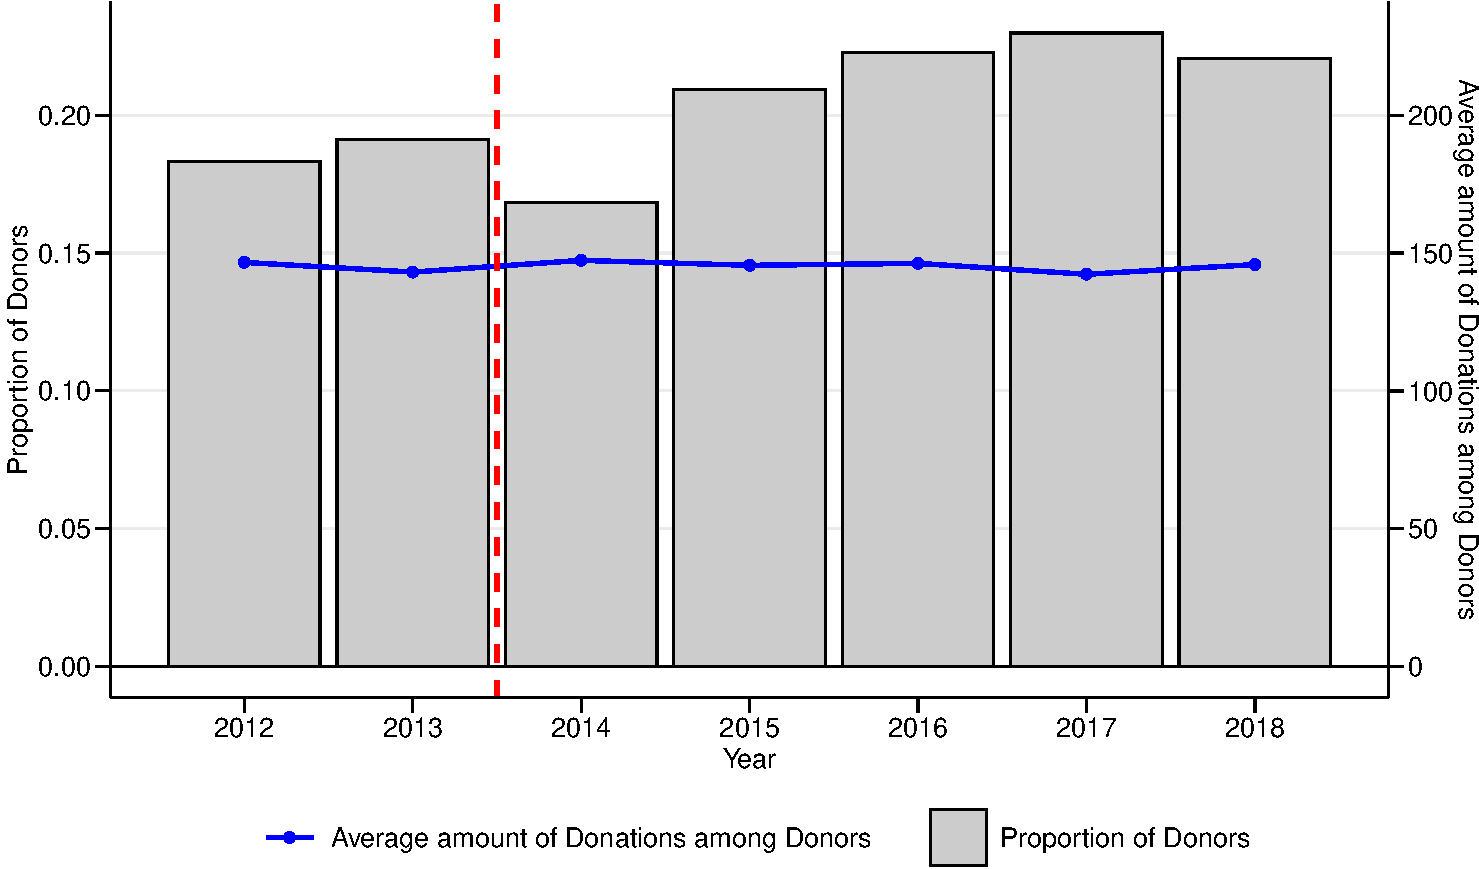
\includegraphics[width=0.9\linewidth]{C:/Users/katoo/Desktop/NASTAB/paper/slide_files/figure-beamer/SummaryOutcome-1} 

}

\caption{Proportion of Donors and Average Donations among Donors. Notes: The left and right axises respectively mesure proportion of donors and the average amount donations among donors. Authors made this graph based on NasTaB data.}\label{fig:SummaryOutcome}
\end{figure}
\end{frame}

\begin{frame}{Income and Giving Price}
\protect\hypertarget{income-and-giving-price}{}
\begin{itemize}
\tightlist
\item
  Figure \ref{fig:SummaryPriceChange} shows the giving price after 2012 and income distribution in 2013.

  \begin{itemize}
  \tightlist
  \item
    Blue line shows the giving price in 2012 and 2013, which depends on income
  \item
    Red dashed line shows the giving price after 2014, which is not a function of income.
  \end{itemize}
\item
  We can make three groups in terms of the benefit from the 2014 tax reform.

  \begin{itemize}
  \tightlist
  \item
    Benefit group: Final taxable income is less than \(1200 \times 10^4\)KRW.
  \item
    Neutral group: Final taxable income lies between \((1200 \times 10^4, 4600 \times 10^4)\).
  \item
    Loss group: Final taxable income is more than \(4600 \times 10^4\)KRW.
  \end{itemize}
\end{itemize}
\end{frame}

\begin{frame}{Giving Price and Income Distribution (Cont'd)}
\protect\hypertarget{giving-price-and-income-distribution-contd}{}
\begin{figure}[t]

{\centering 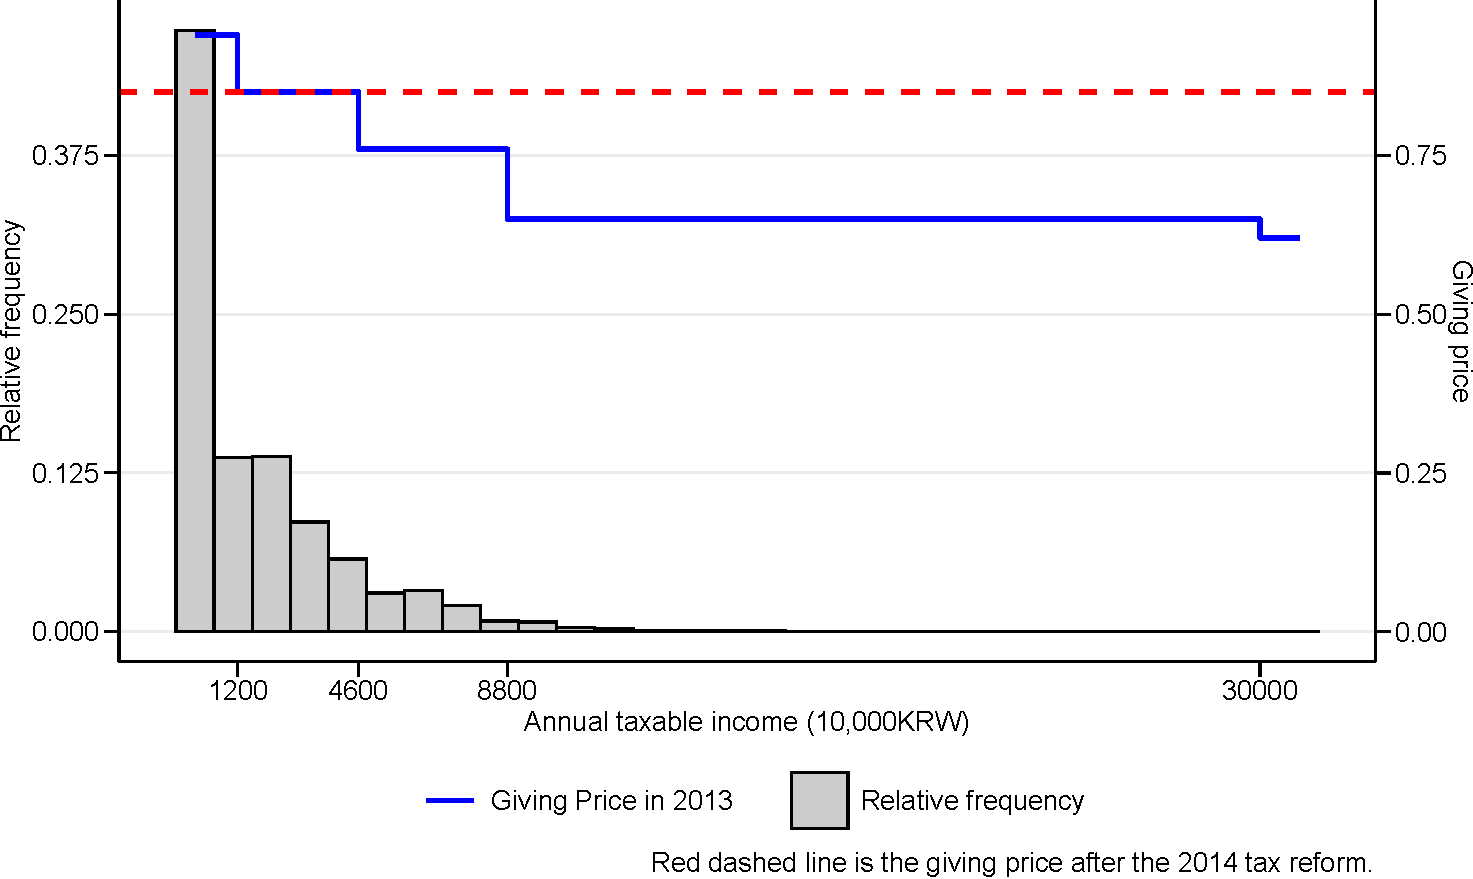
\includegraphics[width=0.9\linewidth]{C:/Users/katoo/Desktop/NASTAB/paper/slide_files/figure-beamer/SummaryPriceChange-1} 

}

\caption{Income Distribution and Giving Price in 2013}\label{fig:SummaryPriceChange}
\end{figure}
\end{frame}

\hypertarget{estimation}{%
\section{Estimation}\label{estimation}}

\begin{frame}{Estimation}
Following Almunia et al. (2020), we estimate giving price elasticity for intensive margin and extensive margin.

\begin{itemize}
\tightlist
\item
  The elasticity of intensive margin shows how much donors additionally donates reacting to the marginal increase of giving price
\item
  The elasticity of extensive margin shows how much the probability to donate changes reacting to marginal increase of giving price.
\end{itemize}
\end{frame}

\begin{frame}{Elasticitiy of Intensive Margin}
\protect\hypertarget{elasticitiy-of-intensive-margin}{}
\[
\ln g_{it} = \varepsilon_{INT} \ln p_{it} +g_{INT} \ln y_{it} + X_{it}\beta +\mu_i +\iota_t +u_{it}. \label{eq:intensive}
\]

\begin{itemize}
\tightlist
\item
  \(g_{it}, p_{it}\) and \(y_{it}\) respectively indicates the amount of giving, the giving price, and income of \(i\) in year \(t\)
\item
  \(\mu_i, \iota_t\) and \(u_{it}\) are individual fixed effect, year fixed effect and error term
\item
  \(X_{it}\) is a vector of covariates which include variables about education and gender. Moreover, we add some interaction terms between year fixed effect and control variables into \(X_{it}\) (following Zeldow and Hatfield (2019)).
\end{itemize}
\end{frame}

\begin{frame}{Elasticitiy of Extensive Margin}
\protect\hypertarget{elasticitiy-of-extensive-margin}{}
\[
D_{it} =  \delta \ln p_{it} +\gamma \ln y_{it} + X_{it}\beta+\mu_i  +\iota_t +v_it. \label{extensive}
\]

\begin{itemize}
\tightlist
\item
  \(D_{it}\) is a dummy variable taking 1 if individual \(i\) donates at year \(t\) and 0 otherwise.
\item
  Since we use linear probability model, \(\delta = \frac{\partial D_{it}}{\partial p_{it}} p_{it}\). The extensive-margin price elasticity is \(\varepsilon_{EXT} = \hat{\delta}/D_{it}\). Thus, we evaluate it at sample mean of \(D_{it}\).
\end{itemize}
\end{frame}

\begin{frame}{Identification Strategy}
\protect\hypertarget{identification-strategy}{}
Our identification assumption is \textbf{the within price variation is exogenous}.

\begin{itemize}
\tightlist
\item
  This is because we use the fixed effect model to obtain elasticities.
\item
  Our identification assumption may hold because the major \emph{within} price variation depends on the 2014 tax reform.

  \begin{itemize}
  \tightlist
  \item
    After tax reform, the giving price is constant across individuals and there is no room for manipulation by donations and income.
  \item
    Before tax reform (2012 and 2013), the giving price depends on (A) endogeneity of giving price and (B) simultaneous determination of income and donations. For these two reasons, the \emph{within} price is partly endogenous.
  \end{itemize}
\end{itemize}
\end{frame}

\begin{frame}{Obstacles for Identification}
\protect\hypertarget{obstacles-for-identification}{}
Our identification assumption may violate due to two endogenous problems under the tax deduction system.

\begin{enumerate}
\tightlist
\item
  Endogeneity of giving price:

  \begin{itemize}
  \tightlist
  \item
    The tax payer can reduce their giving price by increasing their amount of donation and shifting themselves to the lower tax bracket in the tax deduction system.
  \item
    Since this issue does not happen for the first one unit of donation, whose price (``first price'') cannot be changed by adjusting the donation, we use this first price as the giving price in the estimation.
  \end{itemize}
\end{enumerate}
\end{frame}

\begin{frame}{Obstacles for Identification (Cont'd)}
\protect\hypertarget{obstacles-for-identification-contd}{}
Our identification assumption may violate due to two endogenous problems under the tax deduction system.

\begin{enumerate}
\setcounter{enumi}{1}
\tightlist
\item
  Simultaneous determination of income and donations:

  \begin{itemize}
  \tightlist
  \item
    The change of income caused by the tax reform have effects on both donations through the income effect and the giving price through the marginal tax rate.
  \item
    We employ lagged values of taxable income and construct an instrument variable, \(\ln (p_{it}(y_{it-k} - g_{it-k})/p_{it-k}(y_{it-k} - g_{it-k}))\) where \(g_{it-k} = 0\).
  \item
    By fixing income at year \(t - k\), the instrument isolates changes in price from income responses to the tax reform.
  \end{itemize}
\end{enumerate}
\end{frame}

\hypertarget{main-results}{%
\section{Main Results}\label{main-results}}

\begin{frame}{Price and Income Elasticity}
\protect\hypertarget{price-and-income-elasticity}{}
We found the \textbf{price effect} of giving (1\% price increase leads to about 1.1\% giving decrease),
and the \textbf{income effect} of giving(1\% income increase leads to about 5\% giving increase).

\begin{table}

\caption{\label{tab:MainOverall}Main Results: Overall Elasticity of First Price}
\centering
\fontsize{7}{9}\selectfont
\begin{threeparttable}
\begin{tabular}[t]{lccccc}
\toprule
 & (1) & (2) & (3) & (4) & (5)\\
\midrule
ln(giving price) & -1.072*** & -1.264*** & -1.291*** & -1.114*** & -1.241***\\
 & (0.202) & (0.213) & (0.230) & (0.229) & (0.227)\\
ln(annual taxable income) & 5.393*** & 5.080*** & 5.047*** & 5.116*** & 4.946***\\
 & (0.970) & (0.964) & (0.964) & (0.966) & (0.949)\\
Individual FE & Y & Y & Y & Y & Y\\
Time FE & Y & Y & Y & Y & Y\\
Age & N & Y & Y & Y & Y\\
Year x Education & N & N & Y & Y & Y\\
Year x Gender & N & N & N & Y & Y\\
Year x Resident Area & N & N & N & N & Y\\
N & 53269 & 53269 & 53267 & 53267 & 53267\\
Adjusted R-squared & 0.526 & 0.526 & 0.526 & 0.527 & 0.530\\
\bottomrule
\end{tabular}
\begin{tablenotes}
\item Notes: $^{*}$ $p < 0.1$, $^{**}$ $p < 0.05$, $^{***}$ $p < 0.01$. Standard errors are clustered at individual level. When controlling age, we alson include its squared term.
\end{tablenotes}
\end{threeparttable}
\end{table}
\end{frame}

\begin{frame}{Intensive and Extensive Margin: Estimation Results}
\protect\hypertarget{intensive-and-extensive-margin-estimation-results}{}
The intensive-margin price elasticity is -0.5 \textasciitilde{} -1\%.

\begin{table}

\caption{\label{tab:MainIntensive}Main Results: Intensive-Margin Elasticity of First Price}
\centering
\fontsize{7}{9}\selectfont
\begin{threeparttable}
\begin{tabular}[t]{lccccc}
\toprule
 & (1) & (2) & (3) & (4) & (5)\\
\midrule
ln(giving price) & -0.593*** & -0.838*** & -1.016*** & -0.893*** & -0.904***\\
 & (0.203) & (0.212) & (0.232) & (0.243) & (0.249)\\
ln(annual taxable income) & 2.015*** & 1.562** & 1.445** & 1.528** & 1.571**\\
 & (0.675) & (0.655) & (0.647) & (0.651) & (0.653)\\
Individual FE & Y & Y & Y & Y & Y\\
Time FE & Y & Y & Y & Y & Y\\
Age & N & Y & Y & Y & Y\\
Year x Education & N & N & Y & Y & Y\\
Year x Gender & N & N & N & Y & Y\\
Year x Resident Area & N & N & N & N & Y\\
N & 11637 & 11637 & 11637 & 11637 & 11637\\
Adjusted R-squared & 0.675 & 0.675 & 0.676 & 0.676 & 0.678\\
\bottomrule
\end{tabular}
\begin{tablenotes}
\item Notes: $^{*}$ $p < 0.1$, $^{**}$ $p < 0.05$, $^{***}$ $p < 0.01$. Standard errors are clustered at individual level. When controlling age, we alson include its squared term.
\end{tablenotes}
\end{threeparttable}
\end{table}
\end{frame}

\begin{frame}{Intensive and Extensive Margin: Estimation Results}
\protect\hypertarget{intensive-and-extensive-margin-estimation-results-1}{}
The extensive-margin price elasticity is -1.2 \textasciitilde{} -1.4\%.

\begin{table}

\caption{\label{tab:MainExtensive}Main Results: Extensive-Margin Elasticity of First Price}
\centering
\fontsize{7}{9}\selectfont
\begin{threeparttable}
\begin{tabular}[t]{lccccc}
\toprule
 & (1) & (2) & (3) & (4) & (5)\\
\midrule
ln(giving price) & -0.257*** & -0.288*** & -0.273*** & -0.237*** & -0.267***\\
 & (0.046) & (0.048) & (0.052) & (0.052) & (0.051)\\
ln(annual taxable income) & 1.175*** & 1.124*** & 1.125*** & 1.139*** & 1.102***\\
 & (0.223) & (0.223) & (0.223) & (0.224) & (0.220)\\
 &  &  &  &  & \\
Implied price elasticity & -1.176*** & -1.320*** & -1.250*** & -1.086*** & -1.221***\\
 & (0.210) & (0.221) & (0.239) & (0.238) & (0.235)\\
Implied income elasticity & 5.379*** & 5.145*** & 5.148*** & 5.212*** & 5.045***\\
 & (1.023) & (1.021) & (1.023) & (1.024) & (1.005)\\
Individual FE & Y & Y & Y & Y & Y\\
Time FE & Y & Y & Y & Y & Y\\
Age & N & Y & Y & Y & Y\\
Year x Education & N & N & Y & Y & Y\\
Year x Gender & N & N & N & Y & Y\\
Year x Resident Area & N & N & N & N & Y\\
N & 53269 & 53269 & 53267 & 53267 & 53267\\
Adjusted R-squared & 0.458 & 0.458 & 0.458 & 0.458 & 0.462\\
\bottomrule
\end{tabular}
\begin{tablenotes}
\item Notes: $^{*}$ $p < 0.1$, $^{**}$ $p < 0.05$, $^{***}$ $p < 0.01$. Standard errors are clustered at individual level. When controlling age, we alson include its squared term. The implied extensive-marign price elasticity is evaluated at the sample mean of $D_{ijt}$.
\end{tablenotes}
\end{threeparttable}
\end{table}
\end{frame}

\begin{frame}{Robustness Check}
\protect\hypertarget{robustness-check}{}
First potential concern: last price elasticity

\begin{itemize}
\tightlist
\item
  Our baseline results show the \textbf{first} price elasticity to avoid the endogeneity of giving price.
\item
  We estimated the \textbf{last} price elasticity, using the Panel IV method.

  \begin{itemize}
  \tightlist
  \item
    The instrument is the first giving price.
  \item
    Note that the last giving price is equal to the first giving price under the tax credit system.
  \end{itemize}
\end{itemize}
\end{frame}

\begin{frame}{Robustness Check 1: Result}
\protect\hypertarget{robustness-check-1-result}{}
Overall last price elasticity increases twofold.

\begin{table}

\caption{\label{tab:LastOverall}Overall Elasticity of Last Price}
\centering
\fontsize{7}{9}\selectfont
\begin{threeparttable}
\begin{tabular}[t]{lccccc}
\toprule
 & (1) & (2) & (3) & (4) & (5)\\
\midrule
ln(last giving price) & -2.421*** & -2.536*** & -2.750*** & -2.529*** & -2.650***\\
 & (0.204) & (0.216) & (0.233) & (0.231) & (0.229)\\
ln(annual taxable income) & 5.258*** & 5.072*** & 4.981*** & 5.058*** & 4.910***\\
 & (0.961) & (0.961) & (0.959) & (0.961) & (0.948)\\
Individual FE & Y & Y & Y & Y & Y\\
Time FE & Y & Y & Y & Y & Y\\
Age & N & Y & Y & Y & Y\\
Year x Education & N & N & Y & Y & Y\\
Year x Gender & N & N & N & Y & Y\\
Year x Resident Area & N & N & N & N & Y\\
N & 52304 & 52304 & 52302 & 52302 & 52302\\
Adjusted R-squared & 0.529 & 0.529 & 0.529 & 0.530 & 0.533\\
\bottomrule
\end{tabular}
\begin{tablenotes}
\item Notes: $^{*}$ $p < 0.1$, $^{**}$ $p < 0.05$, $^{***}$ $p < 0.01$. Standard errors are clustered at individual level. The instumental variable is the first giving price in year $t$. When controlling age, we alson include its squared term.
\end{tablenotes}
\end{threeparttable}
\end{table}
\end{frame}

\begin{frame}{Robustness Check 1: Intensive Margin}
\protect\hypertarget{robustness-check-1-intensive-margin}{}
The intensive-margin last price elasticity lies within the range of the first price elasticity.

\begin{table}

\caption{\label{tab:LastIntensive}Intensive-Margin Elasticity of Last Price}
\centering
\fontsize{7}{9}\selectfont
\begin{threeparttable}
\begin{tabular}[t]{lccccc}
\toprule
 & (1) & (2) & (3) & (4) & (5)\\
\midrule
ln(last giving price) & -0.898*** & -0.961*** & -1.197*** & -0.998*** & -1.074***\\
 & (0.271) & (0.271) & (0.307) & (0.325) & (0.332)\\
ln(annual taxable income) & 2.024*** & 1.638** & 1.460** & 1.530** & 1.572**\\
 & (0.694) & (0.678) & (0.667) & (0.670) & (0.667)\\
Individual FE & Y & Y & Y & Y & Y\\
Time FE & Y & Y & Y & Y & Y\\
Age & N & Y & Y & Y & Y\\
Year x Education & N & N & Y & Y & Y\\
Year x Gender & N & N & N & Y & Y\\
Year x Resident Area & N & N & N & N & Y\\
N & 10672 & 10672 & 10672 & 10672 & 10672\\
Adjusted R-squared & 0.671 & 0.671 & 0.672 & 0.672 & 0.674\\
\bottomrule
\end{tabular}
\begin{tablenotes}
\item Notes: $^{*}$ $p < 0.1$, $^{**}$ $p < 0.05$, $^{***}$ $p < 0.01$. Standard errors are clustered at individual level. The instumental variable is the first giving price in year $t$. When controlling age, we alson include its squared term.
\end{tablenotes}
\end{threeparttable}
\end{table}
\end{frame}

\begin{frame}{Robustness Check 1: Extensive Margin}
\protect\hypertarget{robustness-check-1-extensive-margin}{}
The extensive-margin last price elasticity at sample mean is roughly -3\%.

\begin{table}

\caption{\label{tab:LastExtensive}Extensive-Margin Elasticity of Last Price}
\centering
\fontsize{7}{9}\selectfont
\begin{threeparttable}
\begin{tabular}[t]{lccccc}
\toprule
 & (1) & (2) & (3) & (4) & (5)\\
\midrule
ln(last giving price) & -0.623*** & -0.630*** & -0.644*** & -0.593*** & -0.619***\\
 & (0.046) & (0.049) & (0.053) & (0.052) & (0.052)\\
ln(annual taxable income) & 1.125*** & 1.113*** & 1.103*** & 1.121*** & 1.090***\\
 & (0.221) & (0.223) & (0.223) & (0.223) & (0.220)\\
 &  &  &  &  & \\
Implied price elasticity & -3.052*** & -3.090*** & -3.156*** & -2.907*** & -3.035***\\
 & (0.227) & (0.239) & (0.258) & (0.257) & (0.254)\\
Implied income elasticity & 5.514*** & 5.453*** & 5.407*** & 5.494*** & 5.343***\\
 & (1.084) & (1.092) & (1.092) & (1.095) & (1.078)\\
Individual FE & Y & Y & Y & Y & Y\\
Time FE & Y & Y & Y & Y & Y\\
Age & N & Y & Y & Y & Y\\
Year x Education & N & N & Y & Y & Y\\
Year x Gender & N & N & N & Y & Y\\
Year x Resident Area & N & N & N & N & Y\\
N & 52304 & 52304 & 52302 & 52302 & 52302\\
Adjusted R-squared & 0.464 & 0.464 & 0.464 & 0.465 & 0.469\\
\bottomrule
\end{tabular}
\begin{tablenotes}
\item Notes: $^{*}$ $p < 0.1$, $^{**}$ $p < 0.05$, $^{***}$ $p < 0.01$. Standard errors are clustered at individual level. The instumental variable is the first giving price in year $t$. When controlling age, we alson include its squared term. The implied extensive-marign price elasticity is evaluated at the sample mean of $D_{ijt}$.
\end{tablenotes}
\end{threeparttable}
\end{table}
\end{frame}

\begin{frame}{Robust Check 2}
\protect\hypertarget{robust-check-2}{}
Second potential concern: Price change due to the change of income

\begin{itemize}
\tightlist
\item
  Since the giving price under the tax deduction depends on the change of income, the \emph{within} variation of giving price may be endogenous.
\item
  To resolve this concern, we used the data (i) from 2013 to 2018 or (ii) from 2013 to 2014, and estimated the fixed effect model.

  \begin{itemize}
  \tightlist
  \item
    By this restriction, the \emph{within} price variation of giving price is completely exgonenous.
  \end{itemize}
\end{itemize}
\end{frame}

\begin{frame}{Robustness Check 2: Result}
\protect\hypertarget{robustness-check-2-result}{}
Overall price elasticity is -1 \textasciitilde{} -1.7\%.

\begin{table}

\caption{\label{tab:ShortOverall}Overall Elasticity with Short-Period Panel}
\centering
\fontsize{7}{9}\selectfont
\begin{threeparttable}
\begin{tabular}[t]{lcccc}
\toprule
\multicolumn{1}{c}{ } & \multicolumn{2}{c}{After 2012} & \multicolumn{2}{c}{2013 and 2014} \\
\cmidrule(l{3pt}r{3pt}){2-3} \cmidrule(l{3pt}r{3pt}){4-5}
 & (1) & (2) & (3) & (4)\\
\midrule
ln(giving price) & -1.014*** & -1.286*** & -1.398*** & -1.686***\\
 & (0.255) & (0.290) & (0.289) & (0.338)\\
ln(annual taxable income) & 5.108*** & 4.743*** & 4.013** & 3.035\\
 & (1.009) & (0.990) & (1.948) & (1.992)\\
Individual FE & Y & Y & Y & Y\\
Time FE & Y & Y & Y & Y\\
Other Controls & N & Y & N & Y\\
N & 45994 & 45992 & 14893 & 14893\\
Adjusted R-squared & 0.535 & 0.538 & 0.590 & 0.592\\
\bottomrule
\end{tabular}
\begin{tablenotes}
\item Notes: $^{*}$ $p < 0.1$, $^{**}$ $p < 0.05$, $^{***}$ $p < 0.01$. Standard errors are clustered at individual level. Other controls are age (its squared value), the interaction between year dummies and education dummies, the interaction between year dummies and gender dummies, and the interaction between year dummies and resident area.
\end{tablenotes}
\end{threeparttable}
\end{table}
\end{frame}

\begin{frame}{Robustness Check 2: Intensive Marign}
\protect\hypertarget{robustness-check-2-intensive-marign}{}
The intensive-margin price elasticity is -0.6 \textasciitilde{} -1\%.
In column (3), the price elasticity is statistically insignificant.

\begin{table}

\caption{\label{tab:ShortIntensive}Intensive-Margin Elasticity with Short-Period Panel}
\centering
\fontsize{7}{9}\selectfont
\begin{threeparttable}
\begin{tabular}[t]{lcccc}
\toprule
\multicolumn{1}{c}{ } & \multicolumn{2}{c}{After 2012} & \multicolumn{2}{c}{2013 and 2014} \\
\cmidrule(l{3pt}r{3pt}){2-3} \cmidrule(l{3pt}r{3pt}){4-5}
 & (1) & (2) & (3) & (4)\\
\midrule
ln(giving price) & -0.647*** & -1.129*** & -0.394 & -0.712**\\
 & (0.236) & (0.291) & (0.310) & (0.363)\\
ln(annual taxable income) & 1.943*** & 1.714*** & 1.440 & 1.047\\
 & (0.662) & (0.649) & (2.975) & (3.072)\\
Individual FE & Y & Y & Y & Y\\
Time FE & Y & Y & Y & Y\\
Other Controls & N & Y & N & Y\\
N & 10158 & 10158 & 2922 & 2922\\
Adjusted R-squared & 0.684 & 0.687 & 0.735 & 0.737\\
\bottomrule
\end{tabular}
\begin{tablenotes}
\item Notes: $^{*}$ $p < 0.1$, $^{**}$ $p < 0.05$, $^{***}$ $p < 0.01$. Standard errors are clustered at individual level. Other controls are age (its squared value), the interaction between year dummies and education dummies, the interaction between year dummies and gender dummies, and the interaction between year dummies and resident area.
\end{tablenotes}
\end{threeparttable}
\end{table}
\end{frame}

\begin{frame}{Robustness Check 2: Extensive Marign}
\protect\hypertarget{robustness-check-2-extensive-marign}{}
The extensive-margin price elasticity at sample mean is -1 \textasciitilde{} -2\%.

\begin{table}

\caption{\label{tab:ShortExtensive}Extensive-Margin Elasticity with Short-Period Panel}
\centering
\fontsize{7}{9}\selectfont
\begin{threeparttable}
\begin{tabular}[t]{lcccc}
\toprule
\multicolumn{1}{c}{ } & \multicolumn{2}{c}{After 2012} & \multicolumn{2}{c}{2013 and 2014} \\
\cmidrule(l{3pt}r{3pt}){2-3} \cmidrule(l{3pt}r{3pt}){4-5}
 & (1) & (2) & (3) & (4)\\
\midrule
ln(giving price) & -0.235*** & -0.269*** & -0.331*** & -0.383***\\
 & (0.058) & (0.065) & (0.065) & (0.076)\\
ln(annual taxable income) & 1.093*** & 1.024*** & 0.801* & 0.574\\
 & (0.230) & (0.226) & (0.428) & (0.447)\\
 &  &  &  & \\
Implied price elasticity & -1.064*** & -1.217*** & -1.689*** & -1.951***\\
 & (0.262) & (0.294) & (0.333) & (0.387)\\
Implied income elasticity & 4.951*** & 4.638*** & 4.082* & 2.926\\
 & (1.043) & (1.024) & (2.181) & (2.279)\\
Individual FE & Y & Y & Y & Y\\
Time FE & Y & Y & Y & Y\\
Other Controls & N & Y & N & Y\\
N & 45994 & 45992 & 14893 & 14893\\
Adjusted R-squared & 0.465 & 0.469 & 0.524 & 0.525\\
\bottomrule
\end{tabular}
\begin{tablenotes}
\item Notes: $^{*}$ $p < 0.1$, $^{**}$ $p < 0.05$, $^{***}$ $p < 0.01$. Standard errors are clustered at individual level. Other controls are age (its squared value), the interaction between year dummies and education dummies, the interaction between year dummies and gender dummies, and the interaction between year dummies and resident area. The implied extensive-marign price elasticity is evaluated at the sample mean of $D_{ijt}$.
\end{tablenotes}
\end{threeparttable}
\end{table}
\end{frame}

\begin{frame}{Robustness Check 3}
\protect\hypertarget{robustness-check-3}{}
Second potential concerns: the change of price due to the change of income

\begin{itemize}
\tightlist
\item
  To exclude this potential concerns, previous identification strategy uses the 2014 tax reform.
\item
  We can also rule out this problem, using the change in the first giving price.

  \begin{itemize}
  \tightlist
  \item
    The change in the first giving price is \(\ln(p_{it}(y_{it-k} - g_{it-k})/p_{it-k}(y_{it-k} - g_{it-k}))\) where \(g_{it-k} = 0\).
  \item
    Since we fix the income \(y_{it-k}\), this variation comes from the tax reform.
  \end{itemize}
\end{itemize}
\end{frame}

\begin{frame}{Robustness Check 3 (Cont'd)}
\protect\hypertarget{robustness-check-3-contd}{}
Our estimation equation is
\[\Delta^k \ln g_{it} = \delta \Delta^k \ln p_{it} + \gamma \Delta^k \ln y_{it} + \Delta^k X_{it} \beta + \mu_i + \iota_t + v_{it},\]
where \(\Delta^k Y_{it} = Y_{it} - Y_{it-k}\).

\begin{itemize}
\tightlist
\item
  Note that we cannot estimation the extensive-margin elasticity since it is hard to interapt this estimation equation when we use \(\Delta^k D_{it}\) as an outcome.
\item
  We estimate this model for \(k = 1, 2, 3\).
\end{itemize}
\end{frame}

\begin{frame}{Robustness Check 3: Overall Elasticity}
\protect\hypertarget{robustness-check-3-overall-elasticity}{}
Overall price elasticity is rougnly -2\%.

\begin{table}

\caption{\label{tab:kdiffOverall}Estimation of Overall Elasticity with $k$-th Difference Model}
\centering
\fontsize{7}{9}\selectfont
\begin{threeparttable}
\begin{tabular}[t]{lccc}
\toprule
 & (1) & (2) & (3)\\
\midrule
1-year lagged difference of first price (log) & -1.894*** &  & \\
 & (0.389) &  & \\
1-year lagged difference of annual income (log) & 2.737*** &  & \\
 & (1.042) &  & \\
2-year lagged difference of first price (log) &  & -2.158*** & \\
 &  & (0.355) & \\
2-year lagged difference of annual income (log) &  & 4.661*** & \\
 &  & (1.139) & \\
3-year lagged difference of first price (log) &  &  & -1.805***\\
 &  &  & (0.345)\\
3-year lagged difference of annual income (log) &  &  & 5.422***\\
 &  &  & (1.181)\\
Individual FE & Y & Y & Y\\
Time FE & Y & Y & Y\\
Other controls & Y & Y & Y\\
N & 49014 & 46587 & 44142\\
Adjusted R-squared & -0.153 & -0.082 & -0.024\\
\bottomrule
\end{tabular}
\begin{tablenotes}
\item Notes: $^{*}$ $p < 0.1$, $^{**}$ $p < 0.05$, $^{***}$ $p < 0.01$. Standard errors are clustered at individual level. The lagged difference of first price (log) is $\ln(\text{Price}^k_{ijt}) - \ln(\text{Price}_{ij(t-k)})$, where $\text{Price}^k_{ijt}$ calculates the giving price under the tax system in year $t$, using annual taxable income in year $t-k$, $\text{Income}_{ij(t-k)}$. The lagged of annual income (log) is $\ln(\text{Income}_{ijt}) - \ln(\text{Income}_{ij(t-k)})$. Other controls are lagged difference of age, lagged difference of squared age, the interaction between year dummies and education dummies, the interaction between year dummies and gender dummies, and the interaction between year dummies and resident area.
\end{tablenotes}
\end{threeparttable}
\end{table}
\end{frame}

\begin{frame}{Robustness Check 3: Intensive-Margin Elasticity}
\protect\hypertarget{robustness-check-3-intensive-margin-elasticity}{}
The intensive-margin price elasticity is rougnly -2\%.

\begin{table}

\caption{\label{tab:kdiffIntensive}Estimation of Intensitve-Margin Elasticity with $k$th Difference Model}
\centering
\fontsize{7}{9}\selectfont
\begin{threeparttable}
\begin{tabular}[t]{lccc}
\toprule
 & (1) & (2) & (3)\\
\midrule
1-year lagged difference of first price (log) & -1.852** &  & \\
 & (0.763) &  & \\
1-year lagged difference of annual income (log) & 2.222 &  & \\
 & (1.715) &  & \\
2-year lagged difference of first price (log) &  & -2.274*** & \\
 &  & (0.621) & \\
2-year lagged difference of annual income (log) &  & 4.601** & \\
 &  & (1.789) & \\
3-year lagged difference of first price (log) &  &  & -2.243***\\
 &  &  & (0.550)\\
3-year lagged difference of annual income (log) &  &  & 5.826***\\
 &  &  & (2.166)\\
Individual FE & Y & Y & Y\\
Time FE & Y & Y & Y\\
Other controls & Y & Y & Y\\
N & 10939 & 10505 & 10040\\
Adjusted R-squared & 0.137 & 0.191 & 0.220\\
\bottomrule
\end{tabular}
\begin{tablenotes}
\item Notes: $^{*}$ $p < 0.1$, $^{**}$ $p < 0.05$, $^{***}$ $p < 0.01$. Standard errors are clustered at individual level. The lagged difference of first price (log) is $\ln(\text{Price}^k_{ijt}) - \ln(\text{Price}_{ij(t-k)})$, where $\text{Price}^k_{ijt}$ calculates the giving price under the tax system in year $t$, using annual taxable income in year $t-k$, $\text{Income}_{ij(t-k)}$. The lagged of annual income (log) is $\ln(\text{Income}_{ijt}) - \ln(\text{Income}_{ij(t-k)})$. Other controls are lagged difference of age, lagged difference of squared age, the interaction between year dummies and education dummies, the interaction between year dummies and gender dummies, and the interaction between year dummies and resident area.
\end{tablenotes}
\end{threeparttable}
\end{table}
\end{frame}

\hypertarget{conclusions}{%
\section{Conclusions}\label{conclusions}}

\begin{frame}{Conclusions}
In this paper, we investigate the giving price elasticity and its heterogeneity as for perception towards the government using South Korean panel data. As a result, we obtain two findings.

Firstly, the estimation shows that the giving price elasticity in Korea is larger than 1 in the sense of absolute value. Although the estimated values seem vulnerable for the estimation method, most of results show that the giving price elasticity is more elastic for extensive margin than intensive margin. This implies that the policymakers should consider not only how much donors additionally pay (intensive margin) but also how many people will be donors (extensive margin) for tax reform.

Secondly, we show that the giving price elasticity for those who think that the government is inefficient is more elastic than the others. Although the previous research shows that those who do not believe the efficiency of the government would donate more than the others, our result firstly shows that such a behavior may depend on the giving price.

From the results, we show that the giving price elasticity would be affected by the efficiency of the government. However, researchers may find the difference of giving behavior as for the other dimensions of heterogeneities. To understand the giving behavior and to contribute the policy making, more sophisticated research is neeeded.

\clearpage
\end{frame}

\hypertarget{references}{%
\section*{References}\label{references}}
\addcontentsline{toc}{section}{References}

\begin{frame}[allowframebreaks]{References}
\hypertarget{refs}{}
\begin{CSLReferences}{1}{0}
\leavevmode\hypertarget{ref-Almunia2020}{}%
Almunia, M., Guceri, I., Lockwood, B., Scharf, K., 2020. More giving or more givers? The effects of tax incentives on charitable donations in the UK. Journal of Public Economics 183. doi:\href{https://doi.org/10.1016/j.jpubeco.2019.104114}{10.1016/j.jpubeco.2019.104114}

\leavevmode\hypertarget{ref-Auten2002}{}%
Auten, G.E., Sieg, H., Clotfelter, C.T., 2002. Charitable giving, income, and taxes: An analysis of panel data. American Economic Review 92, 371--382.

\leavevmode\hypertarget{ref-Bakija2011}{}%
Bakija, J., Heim, B.T., 2011. How does charitable giving respond to incentives and income? New estimates from panel data. National Tax Journal 64, 615--650. doi:\href{https://doi.org/10.17310/ntj.2011.2S.08}{10.17310/ntj.2011.2S.08}

\leavevmode\hypertarget{ref-Fack2010}{}%
Fack, G., Landais, C., 2010. Are tax incentives for charitable giving efficient? Evidence from france. American Economic Journal - Economic Policy 2, 117--141. doi:\href{https://doi.org/10.1257/pol.2.2.117}{10.1257/pol.2.2.117}

\leavevmode\hypertarget{ref-Randolph1995}{}%
Randolph, W.C., 1995. Dynamic income, progressive taxes, and the timing of charitable contributions. Journal of Political Economy 103, 709--738. doi:\href{https://doi.org/10.1086/262000}{10.1086/262000}

\leavevmode\hypertarget{ref-Zeldow2019}{}%
Zeldow, B., Hatfield, L.A., 2019. Confounding and regression adjustment in difference-in-differences. arXiv Preprint.

\end{CSLReferences}
\end{frame}

\end{document}
